\section{Data Handling}\label{subsec:Scaling}
\subsection{Scaling}
The distribution of values for different features can vary immensely, and for most 
cost functions, this is a problem. For some features, a deviation on the magnitude 
of $10^3$ can be a good approximation, whereas for others it can be a vast 
overestimation. When a model is to define which direction it wants to tune, it is 
crucial that the errors across all features are weighted equally. Scaling aims levitate 
this problem by transforming all features to have a relatively equal range of values while
simultaneously preserving all information regarding each feature. The choice of how one 
chooses to scale the data will heavily affect the performance of the model and is therefore
a part of the model. 
\\
\subsubsection{Standard Scaler}
The \emph{Standrad Scaler} implemented in this rapport uses Scikit-learns's \emph{StandardScaler}
\cite{StandardScaler}. The standard scaler function scales each feature individually by subtracting 
the mean and dividing by the standard deviation. In doing so the resulting scaled data has a mean 
of 0 and a standard deviation of 1. Mathematically the standard scaler, $\mathcal{S}$ transforms 
a data set, $X$ as 
\begin{align}
    \mathcal{S} \left(X\right) = \frac{X - \boldsymbol{\mu} _x}{\boldsymbol{\sigma}_x} ,
\end{align}
where $\boldsymbol{\mu} _x$ and $\boldsymbol{\sigma}_x$ are vectors with the elements being 
the mean and standard deviation respectively for each feature.

\subsection{Principal Component Analysis}
\ac{PCA} is a popular dimensionality reduction technique used in many analyses. The goal of
\ac{PCA} is to reduce a high-dimensional dataset while at the same time conserve as much of the 
variance in the data as possible. The motivation behind dimensionality reduction is rooted in 
two (main) reasons. The first being noise reduction. Some features could not only be non-contributing 
during training, but could even introduce noise. The second reason is lack of convergence. In a large 
data set with many features and different classifications (in our case channels), a \ac{ML} could struggle
to identify the most important trends. By reducing the dimensionality in the data, the hope is that this 
would be easier. 
\\
In simple terms, \ac{PCA} finds the direction in the feature space along which the data has the largest 
variance. It does this in 4 steps:
\begin{itemize}
    \item $\textbf{First}$: Center the data around 0 by subtracting the mean from each feature.
    \item $\textbf{Second}$: Calculate the covariance matrix to find the covariance 
                             of each feature pair.
    \item $\textbf{Third}$: Calculate the eigenvalue and eigenvectors of the covariance matrix.
    \item $\textbf{Fourth}$: Order the eigenvector by the eigenvectors to define the directions 
                             in the feature space with the largest variance.
    \item $\textbf{Fifth}$: Cast the data along these directions to form a new data set with 
                             the new features ranked from largest to lowest variance.
    \item $\textbf{Sixth}$: Remove the features with the least variance according to some threshold.                      
\end{itemize}
In figures \ref{fig:PCA1} and \ref{fig:PCA2} I have plotted the distribution of 10, 100 and 500 samples 
for the features with the most and second most variance (\ref{fig:PCA1}), and least and second least 
variance (\ref{fig:PCA2}) after applying \ac{PCA} to our data set. In this \ac{PCA} I am yet to remove features, 
so all four features are taken from a data set where all the variance is still conserved. With this in 
mind, the different scales on the y- and x-axis ($10^0$ for figure \ref{fig:PCA1} and $10^{-7}$ for figure 
\ref{fig:PCA2}) show why we are able to justify removing the features. In figure \ref{fig:PCA2} we observe 
that all channels exhibit the same trends and are practically identical. In other words, these features 
would not contribute in training a model to distinguish the different channels.
\begin{figure}
    \centering
    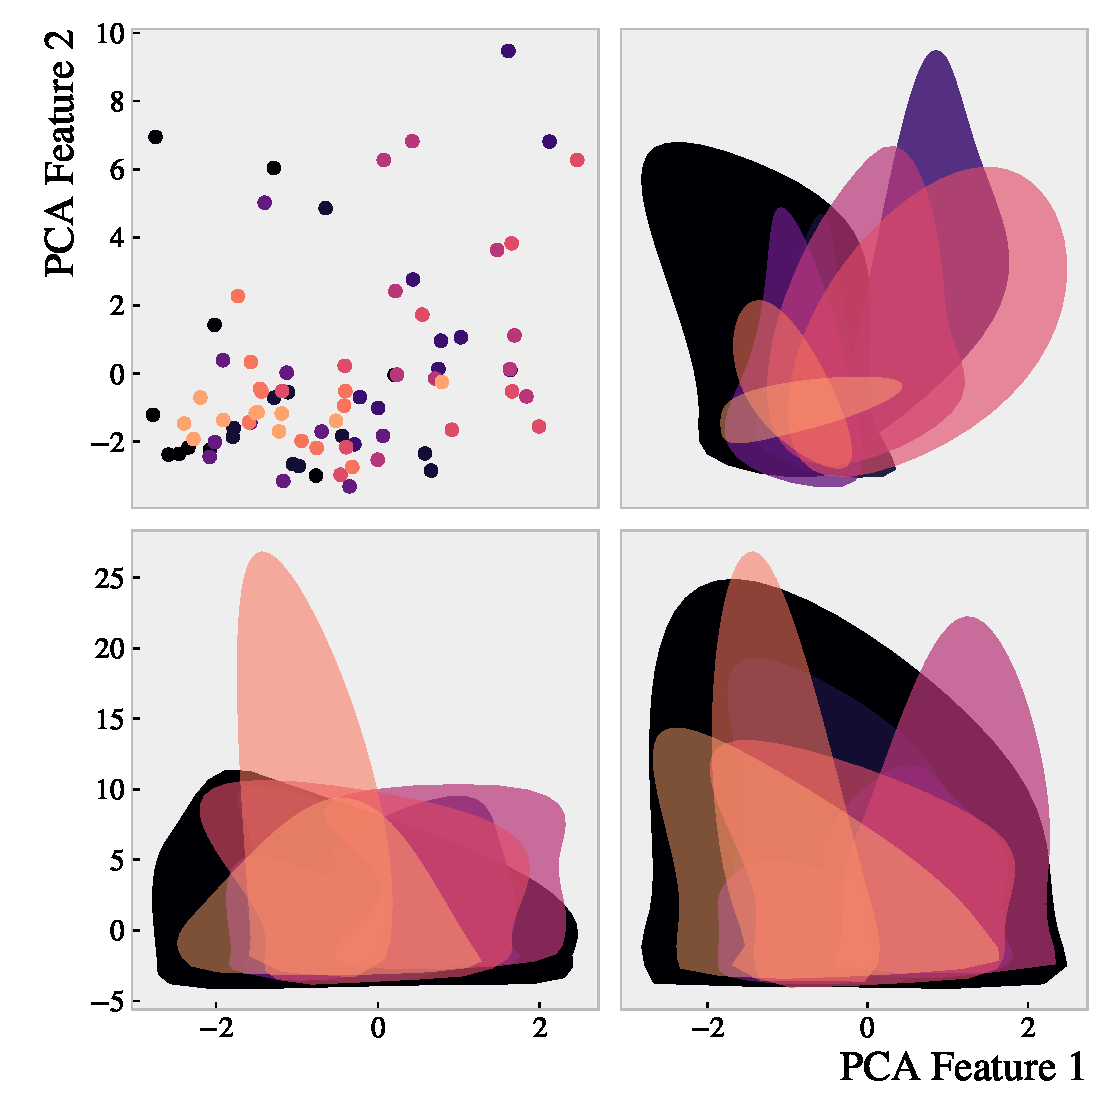
\includegraphics[width=0.6\textwidth]{Figures/MLResults/DataHandling/PCA/PCAPlotFirst.pdf}
    \caption{The distribution of the two PCA-features containing most variation for (left to right, 
    up to down) 10, 10, 100 and 500 samples from each channel. Each sample filling the requirement 
    with being less than one standard deviation from the mean of both features, respectively.}
    \label{fig:PCA1}
\end{figure}
\begin{figure}
    \centering
    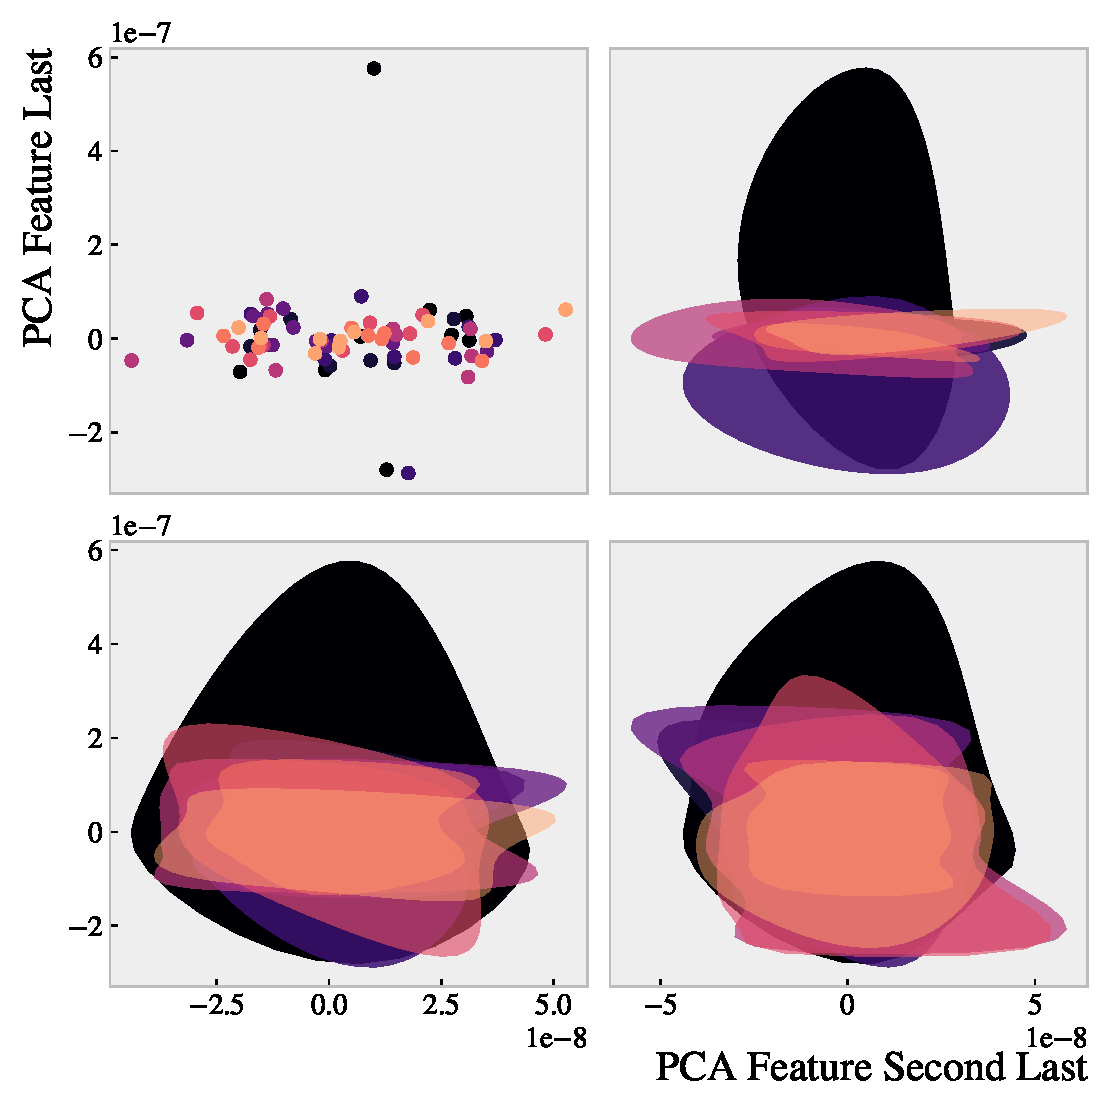
\includegraphics[width=0.6\textwidth]{Figures/MLResults/DataHandling/PCA/PCAPlotLast.pdf}
    \caption{The distribution of the two PCA-features containing the least amount of variation for (left to right, 
    up to down) 10, 10, 100 and 500 samples from each channel. Each sample filling the requirement 
    with being less than one standard deviation from the mean of both features, respectively.}
    \label{fig:PCA2}
\end{figure}


